\subsection{Fact 1: outside FOMC windows, thirty years of yield changes net to zero}

Replicating Hillenbrand (2025) on GSW yields and a hand-built event list: yields move on
non-FOMC days about as much as on FOMC days --- daily standard deviations of 5.60 against
6.72 bp. What differs is that outside the window the moves offset. Across 7{,}035 non-FOMC days
the cumulative change is $-0.82$ pp, a drift of $-0.012$ bp/day with $t = -0.18$; inside
three-day FOMC windows, 11.8\% of trading days, the ten-year fell 6.16 pp of a total 6.99
(Figure~\ref{fig:fact}). A randomisation test placing 324 randomly timed three-day blocks on
non-FOMC days puts the observed figure at the 0th percentile of 5{,}000 draws.

Hillenbrand's explanation is \textbf{long-run Fed guidance}: announcements are the moments at
which the Fed reveals its own estimate of where rates settle in the long run --- implicitly
before 2012, when the rate decision itself disclosed the Committee's read of the natural rate,
and explicitly after 2012 through the SEP longer-run dot. Read through the identity in
\S\ref{sec:framework}, the claim is that in FOMC windows
$\Delta y^{(n)} \approx \Delta r^{*}$, with the inflation anchor, the policy stance and the term
premium all contributing nothing. Those are three separate exclusions, and much of what follows
is about which of them survive.

The distinction between drift and permanence matters for \S\ref{sec:componentB}, which turns on
it: this is a statement about conditional means by day type, not about the permanence of
innovations. The in-window edge is small --- a mean of $-0.63$ bp/day against $-0.01$ elsewhere,
less than a tenth of a daily standard deviation, with 53.4\% of window days negative against
51.5\% of the rest. Nothing about an individual FOMC day looks unusual. The fact is entirely one
of aggregation: 972 window days at $-0.63$ bp compound to $-6.16$ pp, while 7{,}035 other days
at $-0.01$ compound to $-0.82$.

The extension to July 2026 rules out a symmetric reading of the mechanism. Over 2022--2026 the
Fed raised the target 525 bp and revised its own longer-run projection \emph{up} 0.74 pp, and
the ten-year rose 2.60 pp --- but inside FOMC windows it fell 1.20 pp, and the in-window series
continued to decline throughout. Whatever operates in the window did not reverse when policy
did.

\begin{figure}[tbp]
\centering
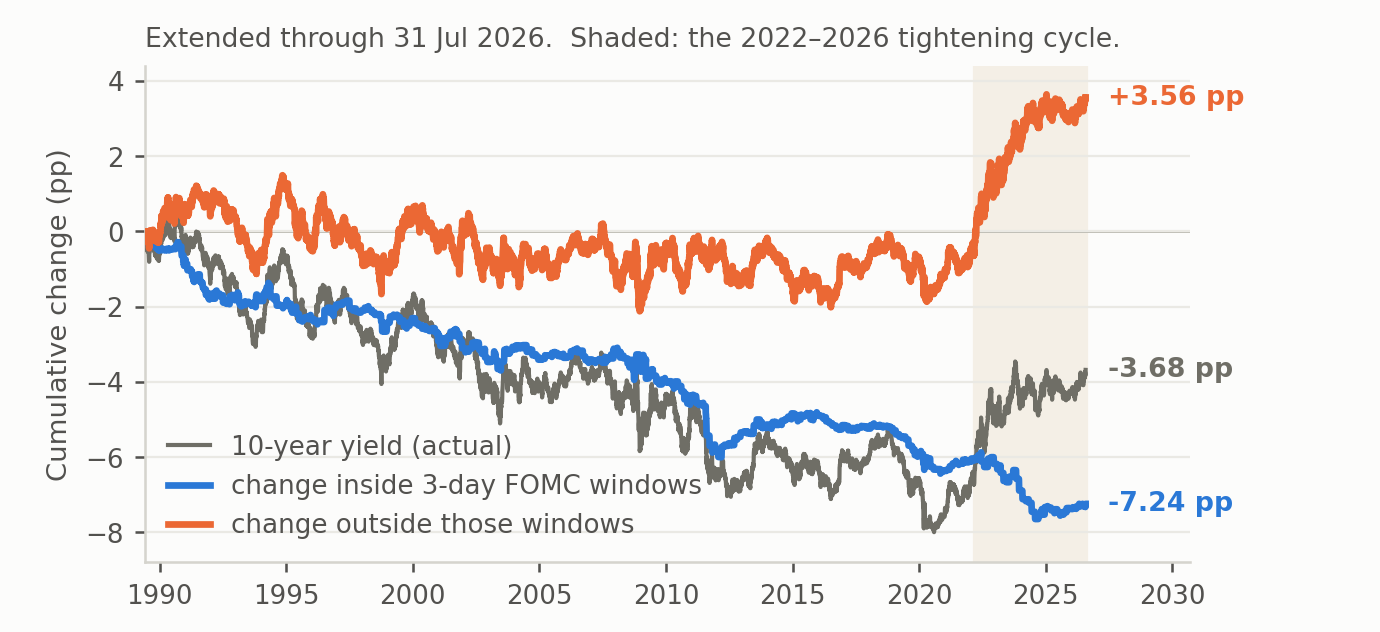
\includegraphics[width=0.86\textwidth]{s_extend.png}
\caption{\textbf{Fact 1.} Cumulative change in the ten-year yield from 2 June 1989, split into
the part accruing inside three-day FOMC windows and the part accruing on all other days,
through 31 July 2026. Shaded: the 2022--2026 tightening cycle.}
\label{fig:fact}
\end{figure}
